
\section{Design}
This section provides an overview of the design aspects of our tool during the second sprint. It includes diagrams that illustrate the system's structure and behavior.

\subsection{Class Diagram}

The class diagram (Figure \ref{fig:Sprint 2 Class Diagram}) visualizes the system's structure. It shows the classes, their attributes and operations, and the relationships among them.

\begin{figure}[ht]
	\centering
	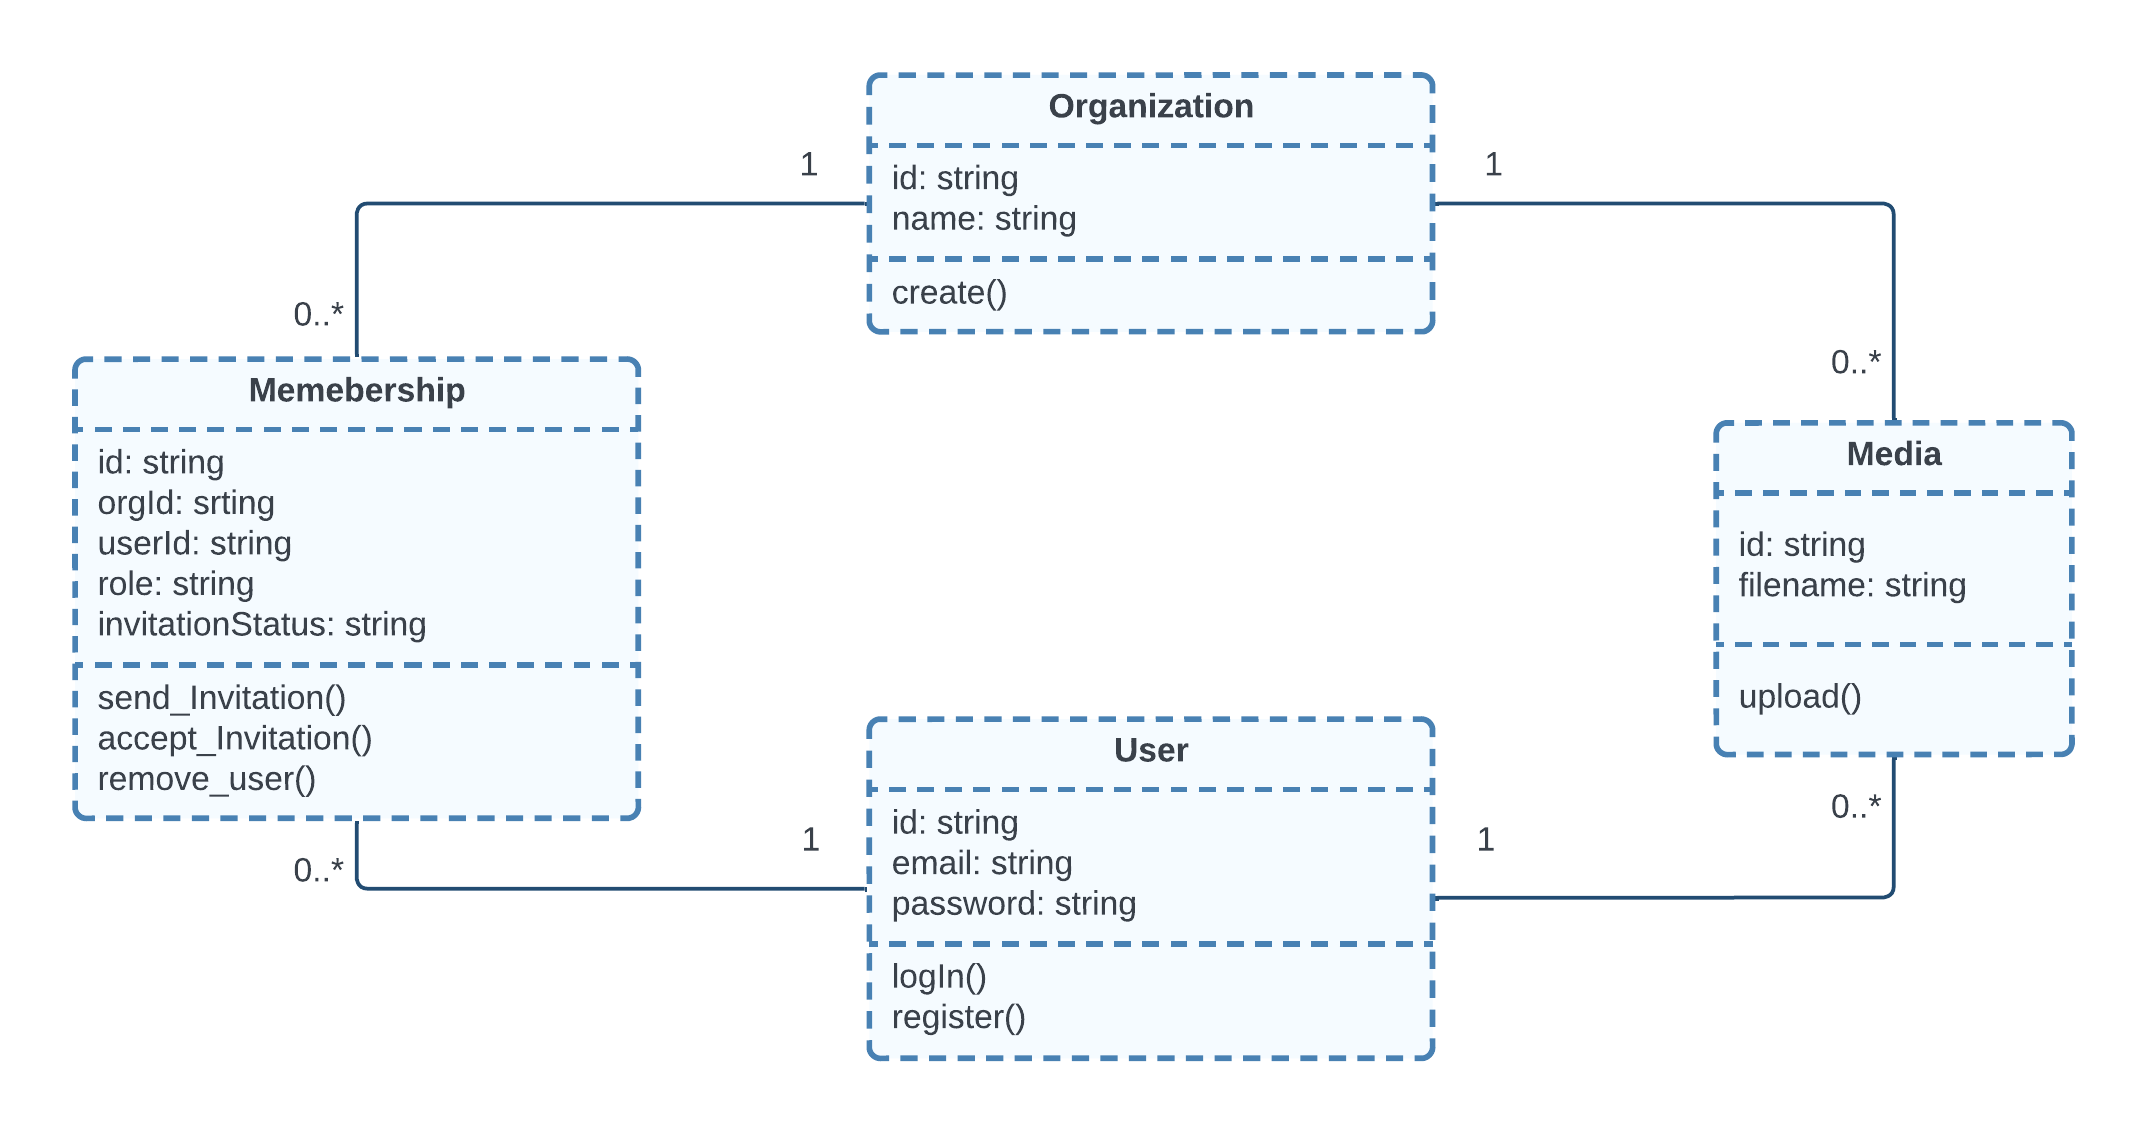
\includegraphics[width=\linewidth]{Images/sprint2/class diagram.png}
	\caption{Sprint 2 Class Diagram}
	\label{fig:Sprint 2 Class Diagram}
\end{figure}

\subsection{Sequence Diagrams}

The sequence diagrams illustrate the flow of operations in the system, emphasizing the interaction between objects over time. Each diagram corresponds to a specific use case or functionality.

\subsubsection{Media Upload Sequence Diagram}

Figure \ref{fig:Sprint 2 Media Upload Sequence Diagram} describes the scenario of the "Media Upload" use case.

\begin{figure}[ht]
	\centering
	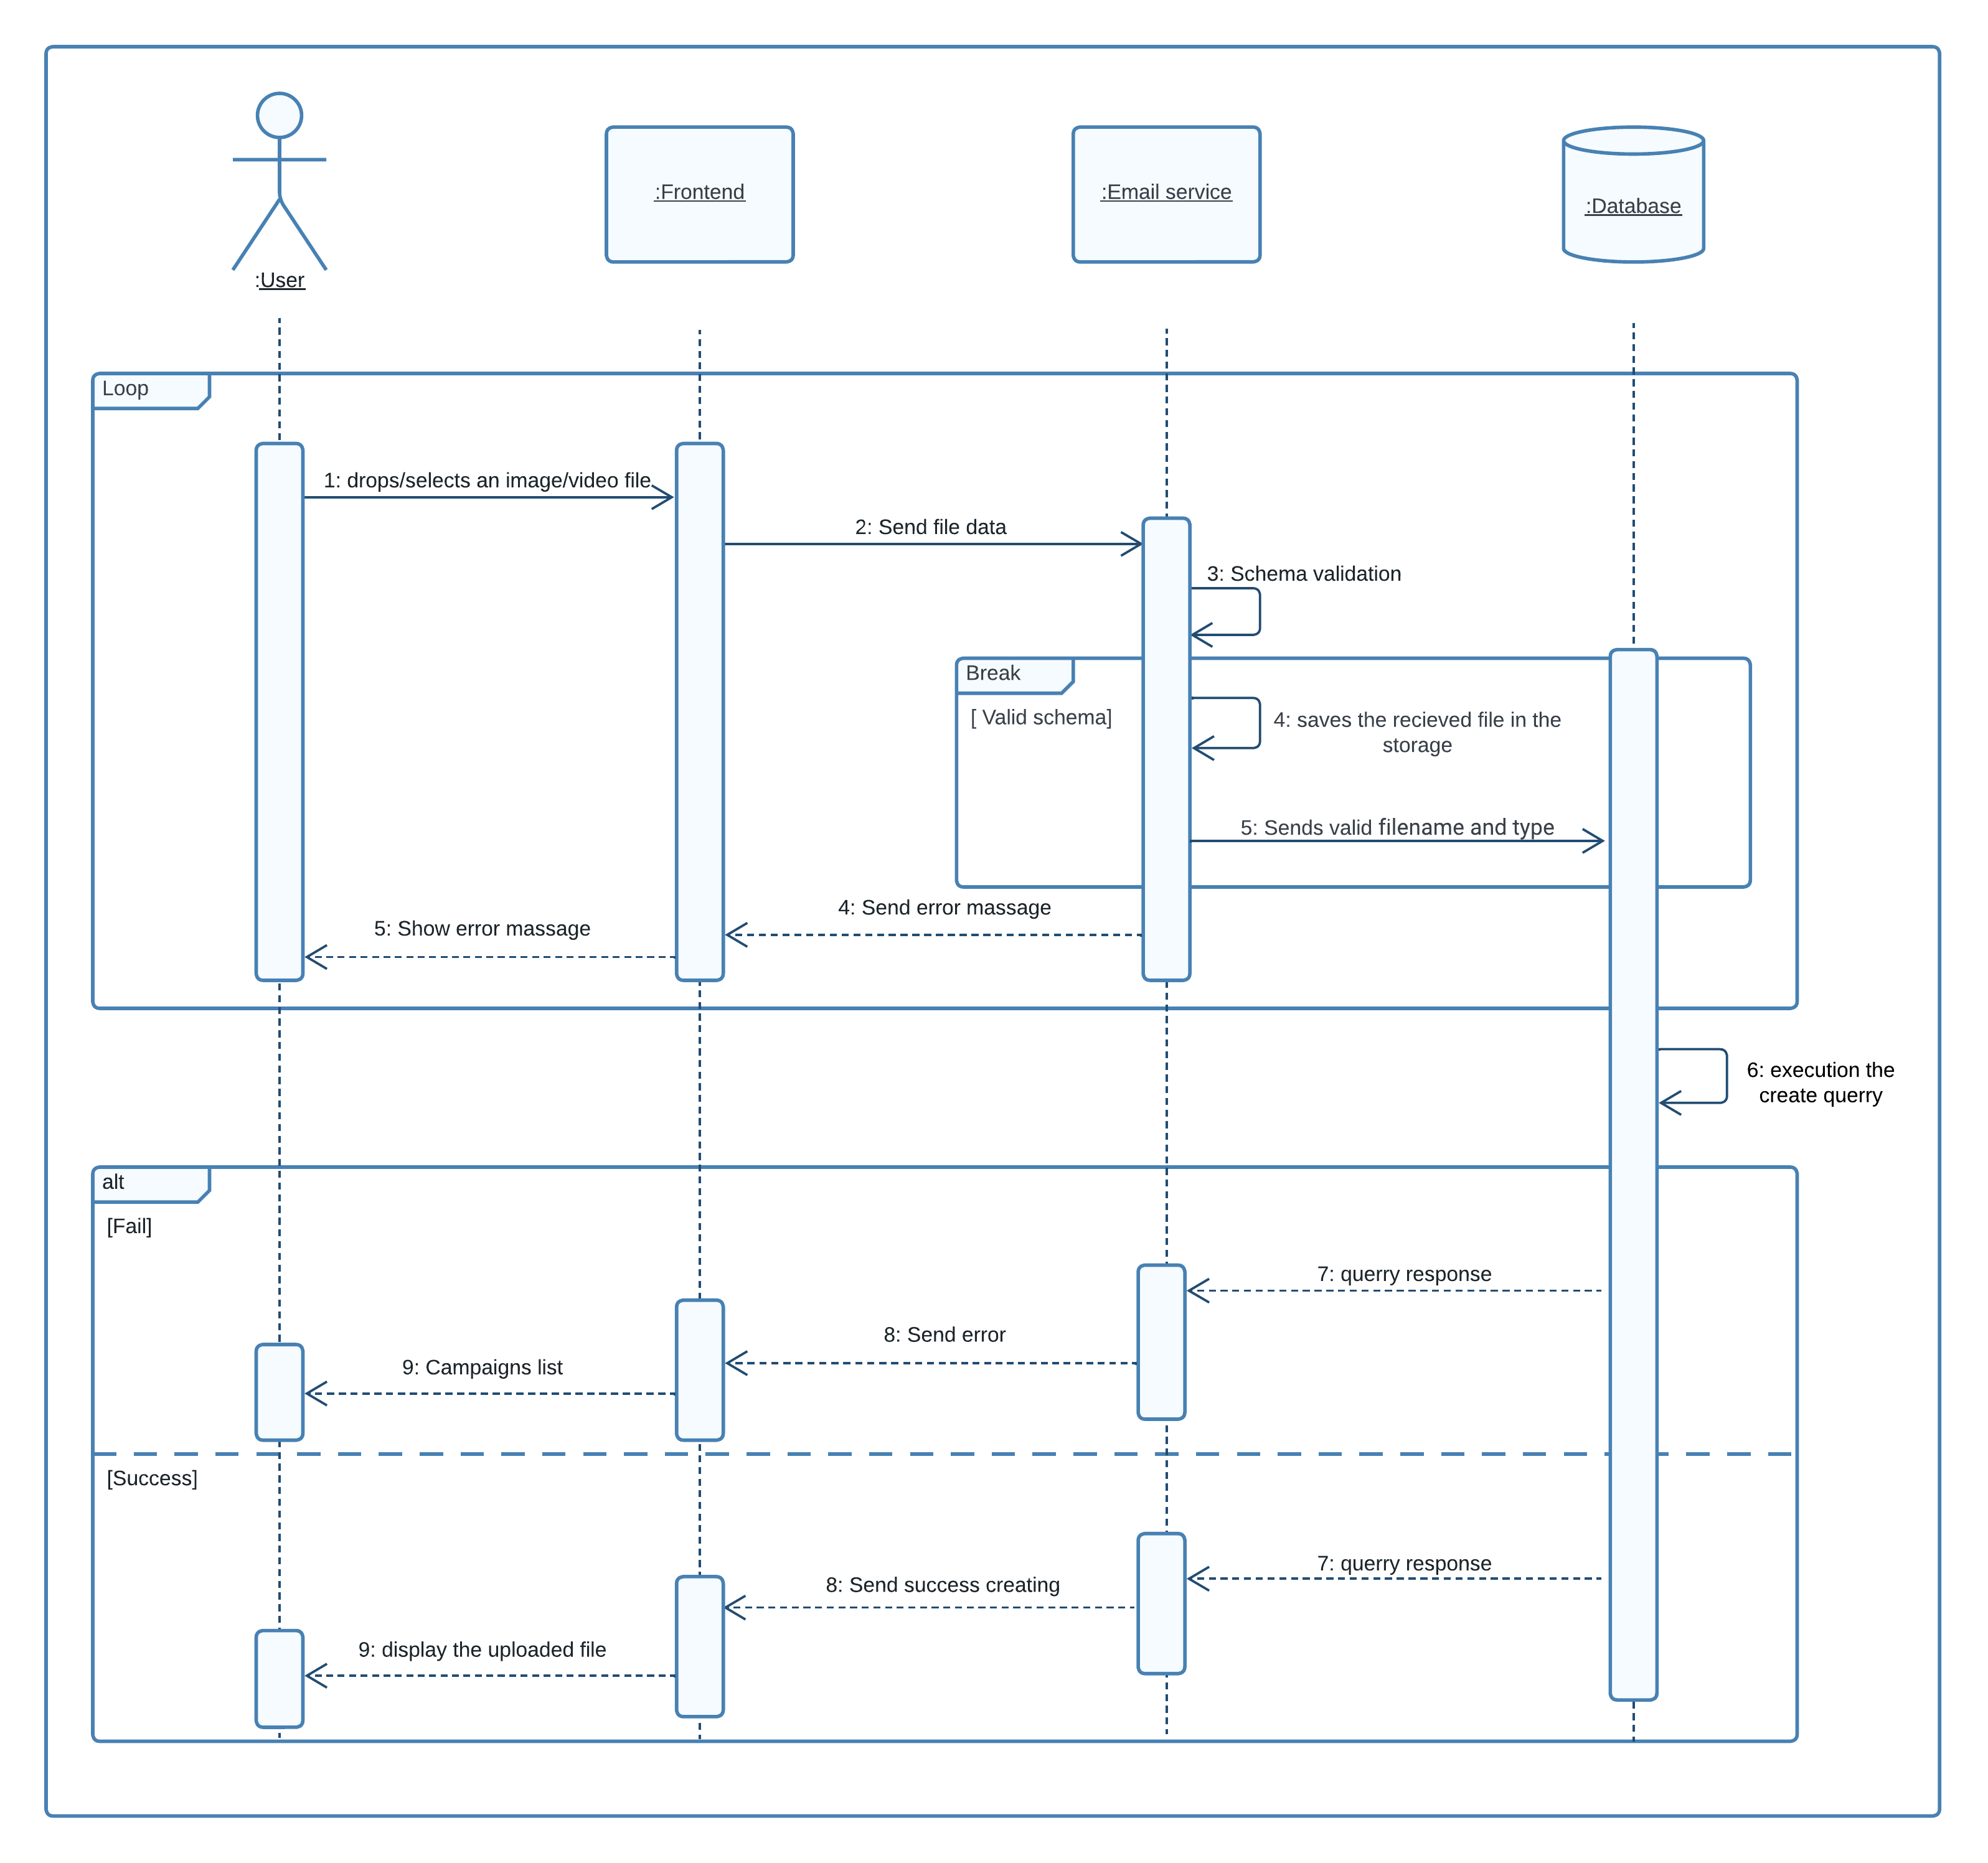
\includegraphics[width=\linewidth]{Images/sprint2/upload media sequence diagram.png}
	\caption{ Media Upload Sequence Diagram}
	\label{fig:Sprint 2 Media Upload Sequence Diagram}
\end{figure}

\clearpage
\subsubsection{Organization Creation Sequence Diagram}

Figure \ref{fig:Sprint 2 Organization Creation Sequence Diagram} describes the scenario of the "Organization Creation" use case.

\begin{figure}[ht]
	\centering
	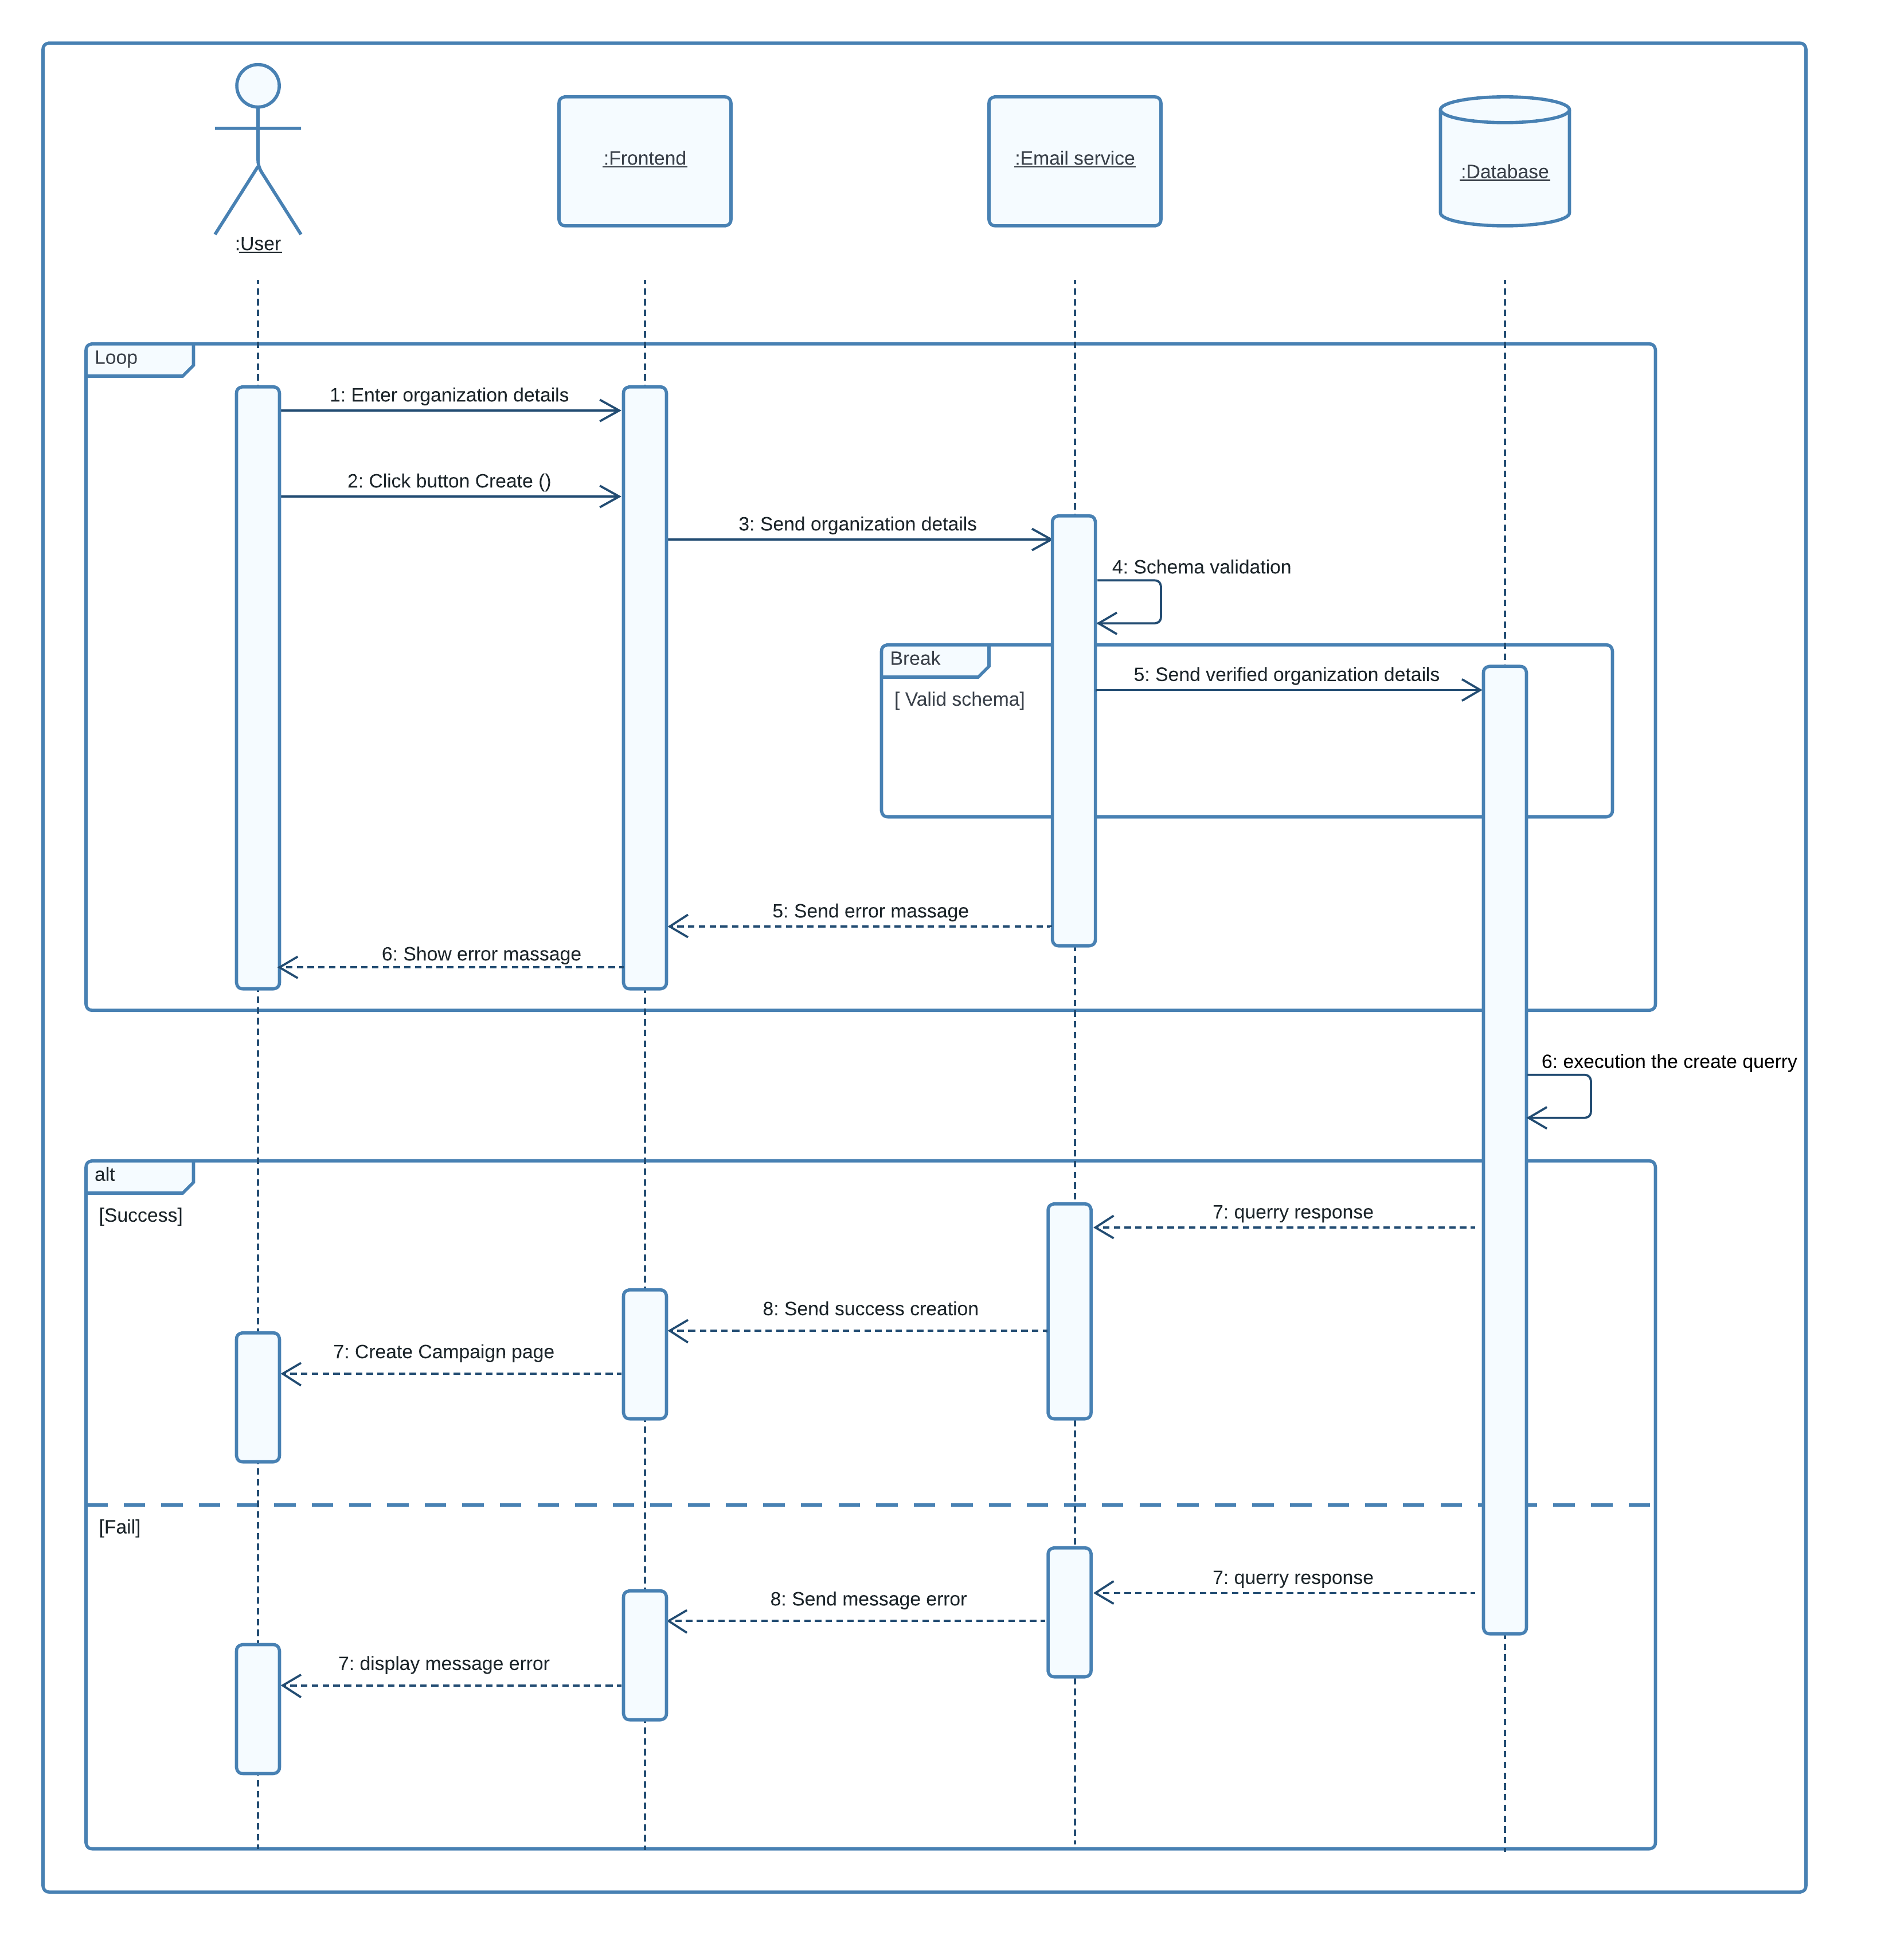
\includegraphics[width=\linewidth]{Images/sprint2/create org sequence diag.png}
	\caption{Organization Creation Sequence Diagram}
	\label{fig:Sprint 2 Organization Creation Sequence Diagram}
\end{figure}

\clearpage

\subsubsection{Send Invitation Sequence Diagram}

Figure \ref{fig:Sprint 2 Send Invitation Sequence Diagram} describes the scenario of the "Send Invitation" use case.

\begin{figure}[ht]
	\centering
	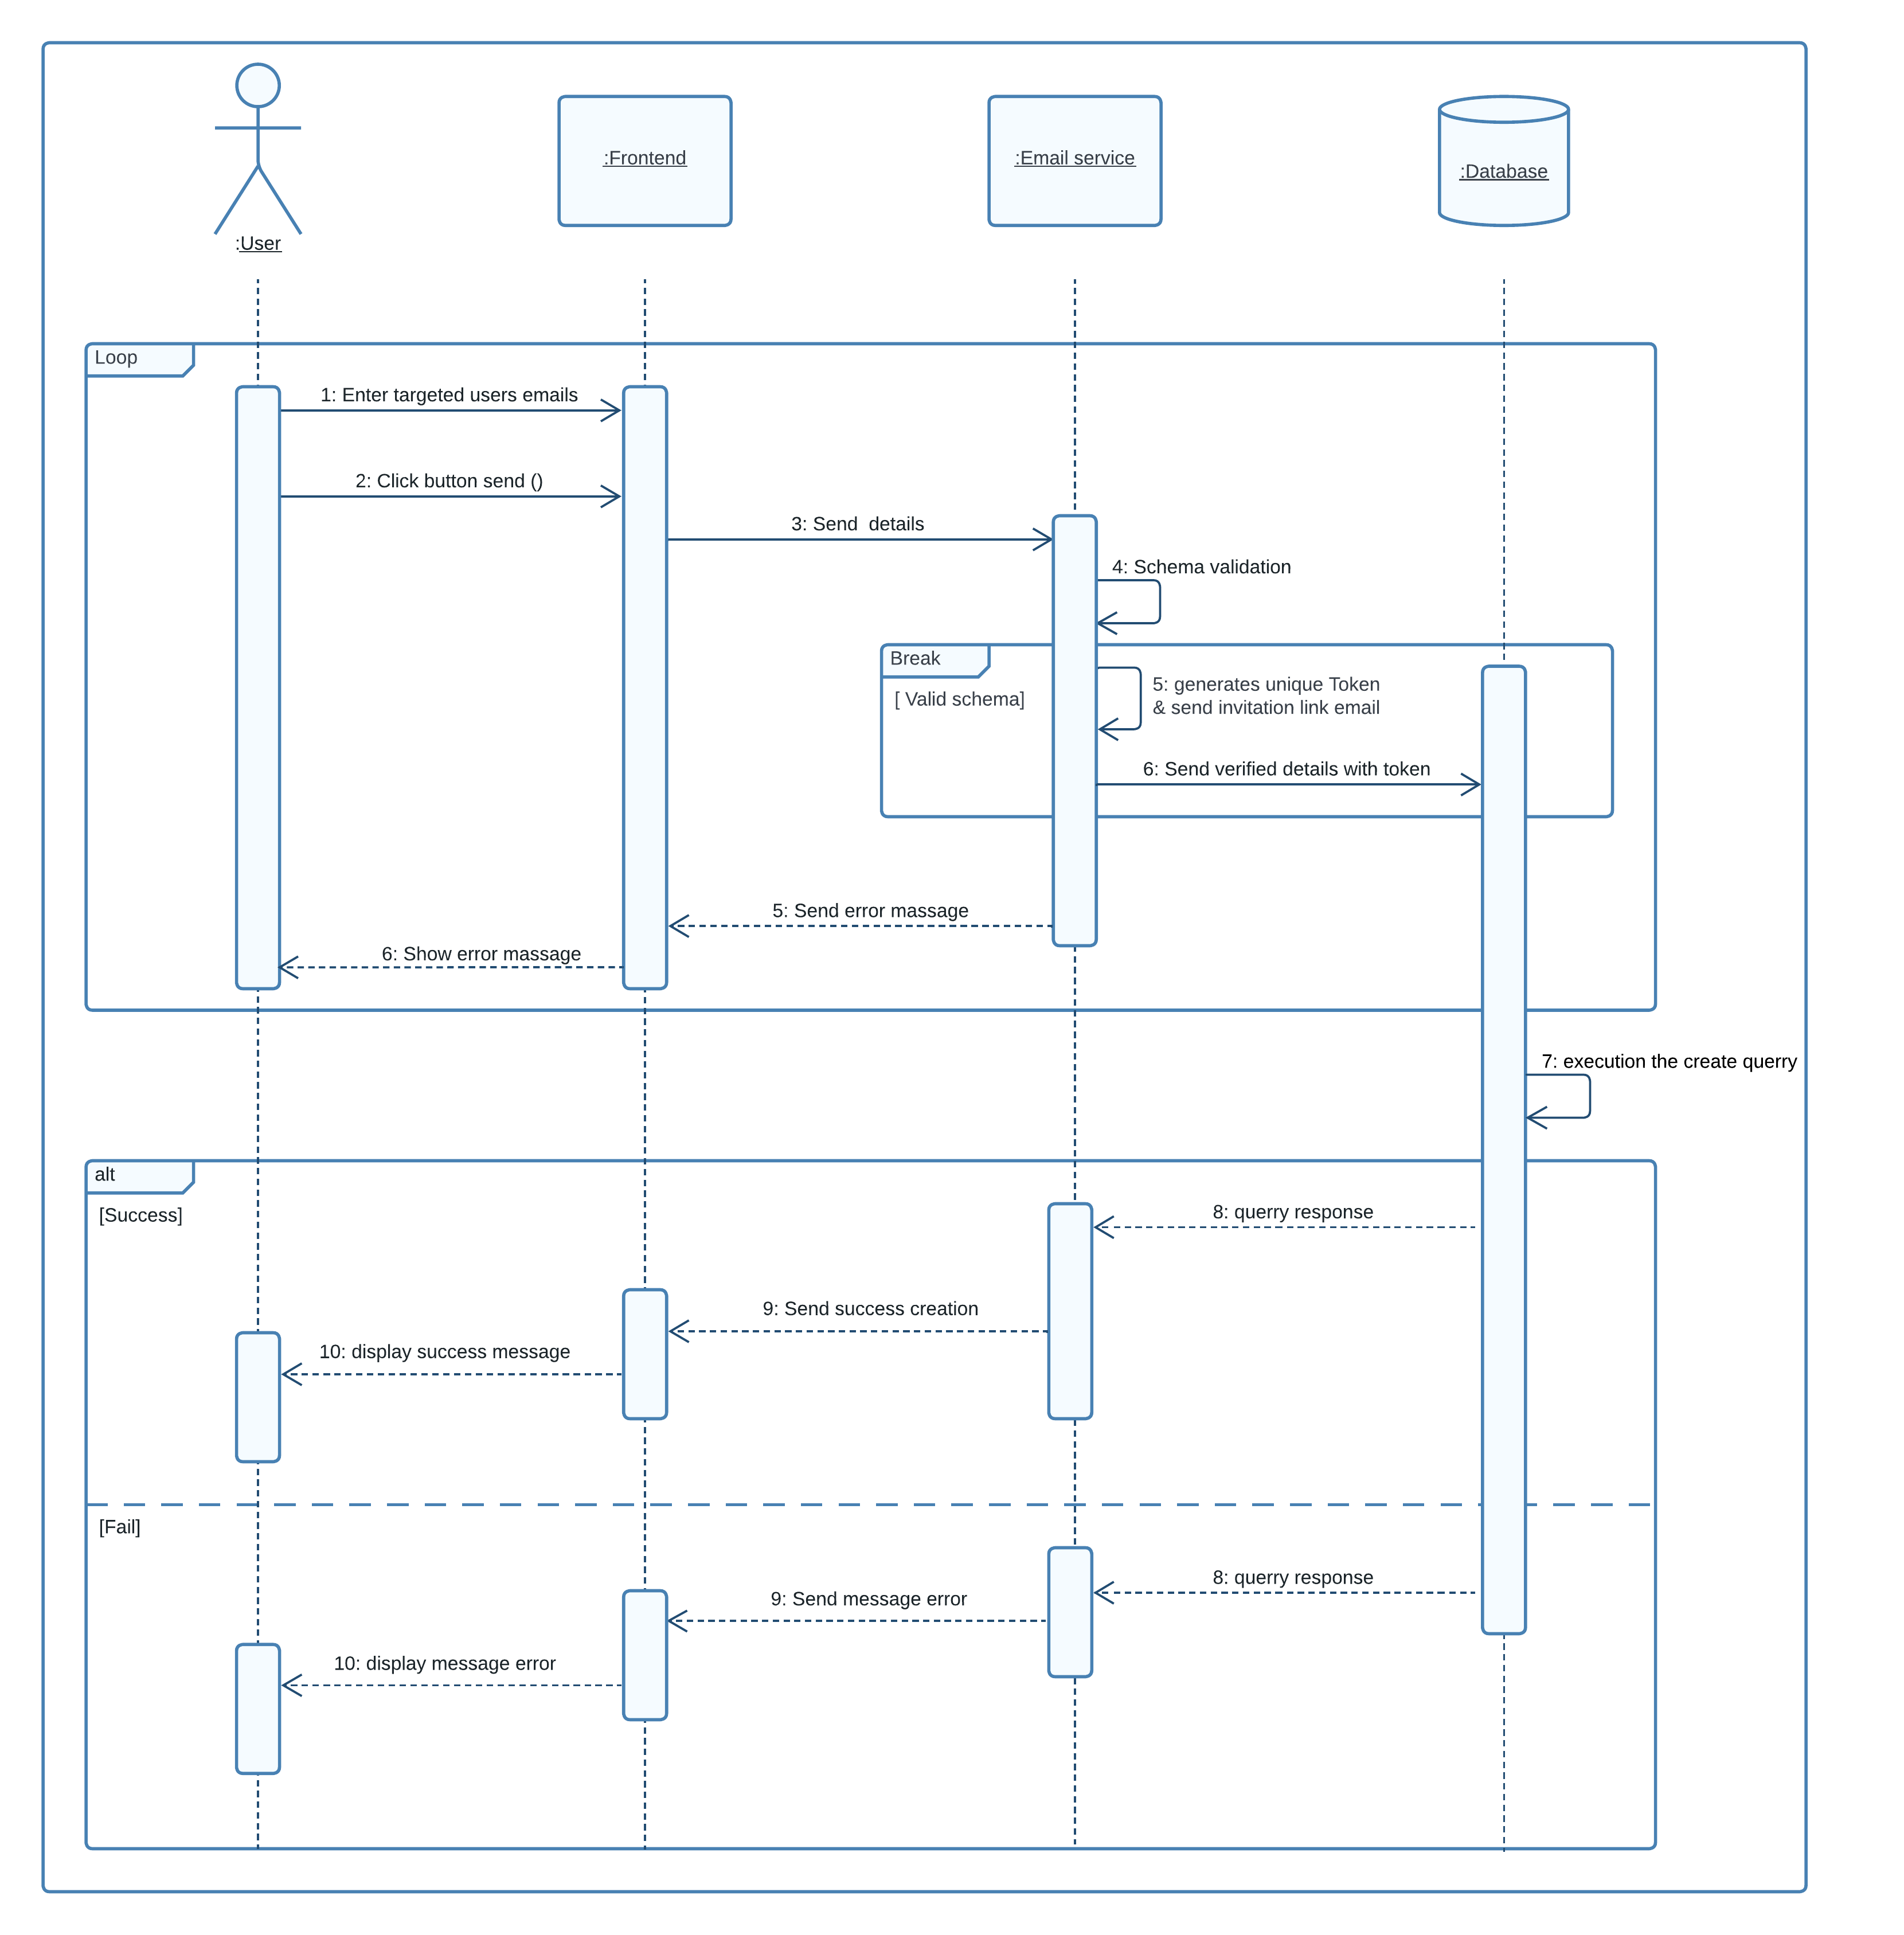
\includegraphics[width=\linewidth]{Images/sprint2/send invitation seq diag.png}
	\caption{ Send Invitation Sequence Diagram}
	\label{fig:Sprint 2 Send Invitation Sequence Diagram}
\end{figure}


\clearpage
\subsubsection{Accept Invitation Sequence Diagram}

Figure \ref{fig:Sprint 2 Accept Invitation Sequence Diagram} describes the scenario of the "Accept Invitation" use case.

\begin{figure}[ht]
	\centering
	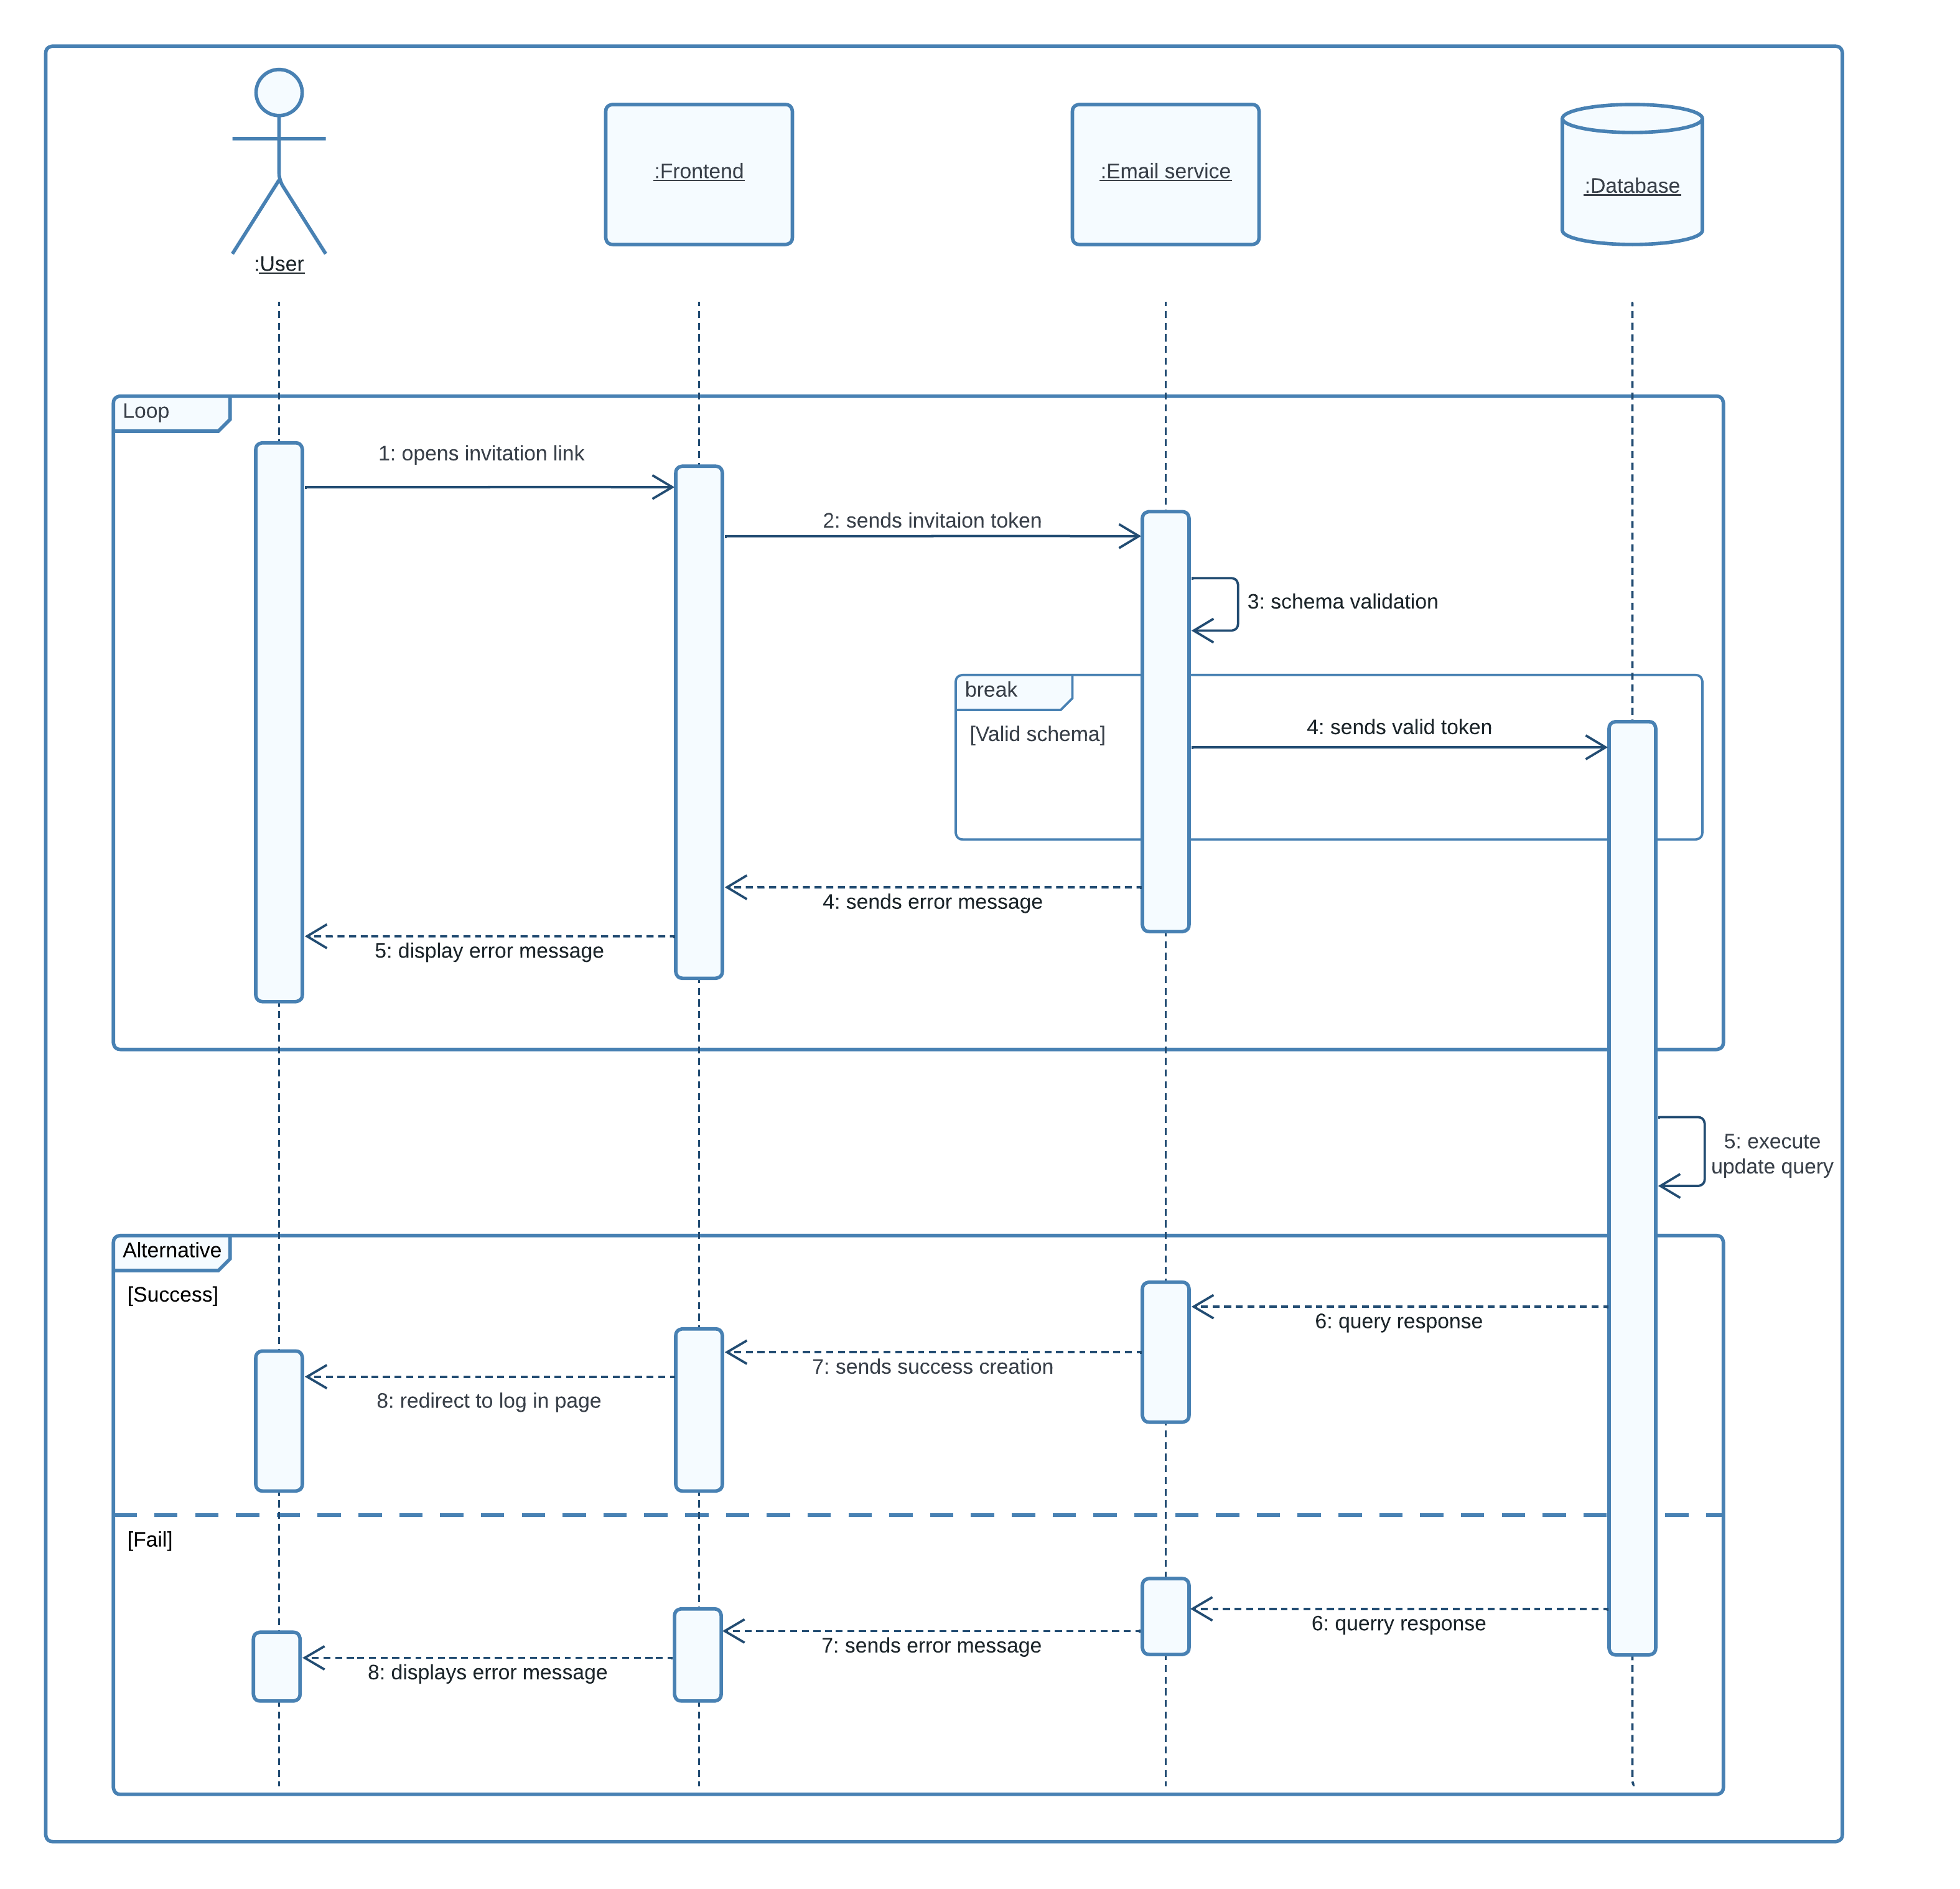
\includegraphics[width=\linewidth]{Images/sprint2/accept invitation sequence diag.png}
	\caption{ Accept Invitation Sequence Diagram}
	\label{fig:Sprint 2 Accept Invitation Sequence Diagram}
\end{figure}

\clearpage

\subsubsection{Assign Roles Sequence Diagram}

Figure \ref{fig:Sprint 2 Assign Roles Sequence Diagram} describes the scenario of the "Assign Roles" use case.

\begin{figure}[ht]
	\centering
	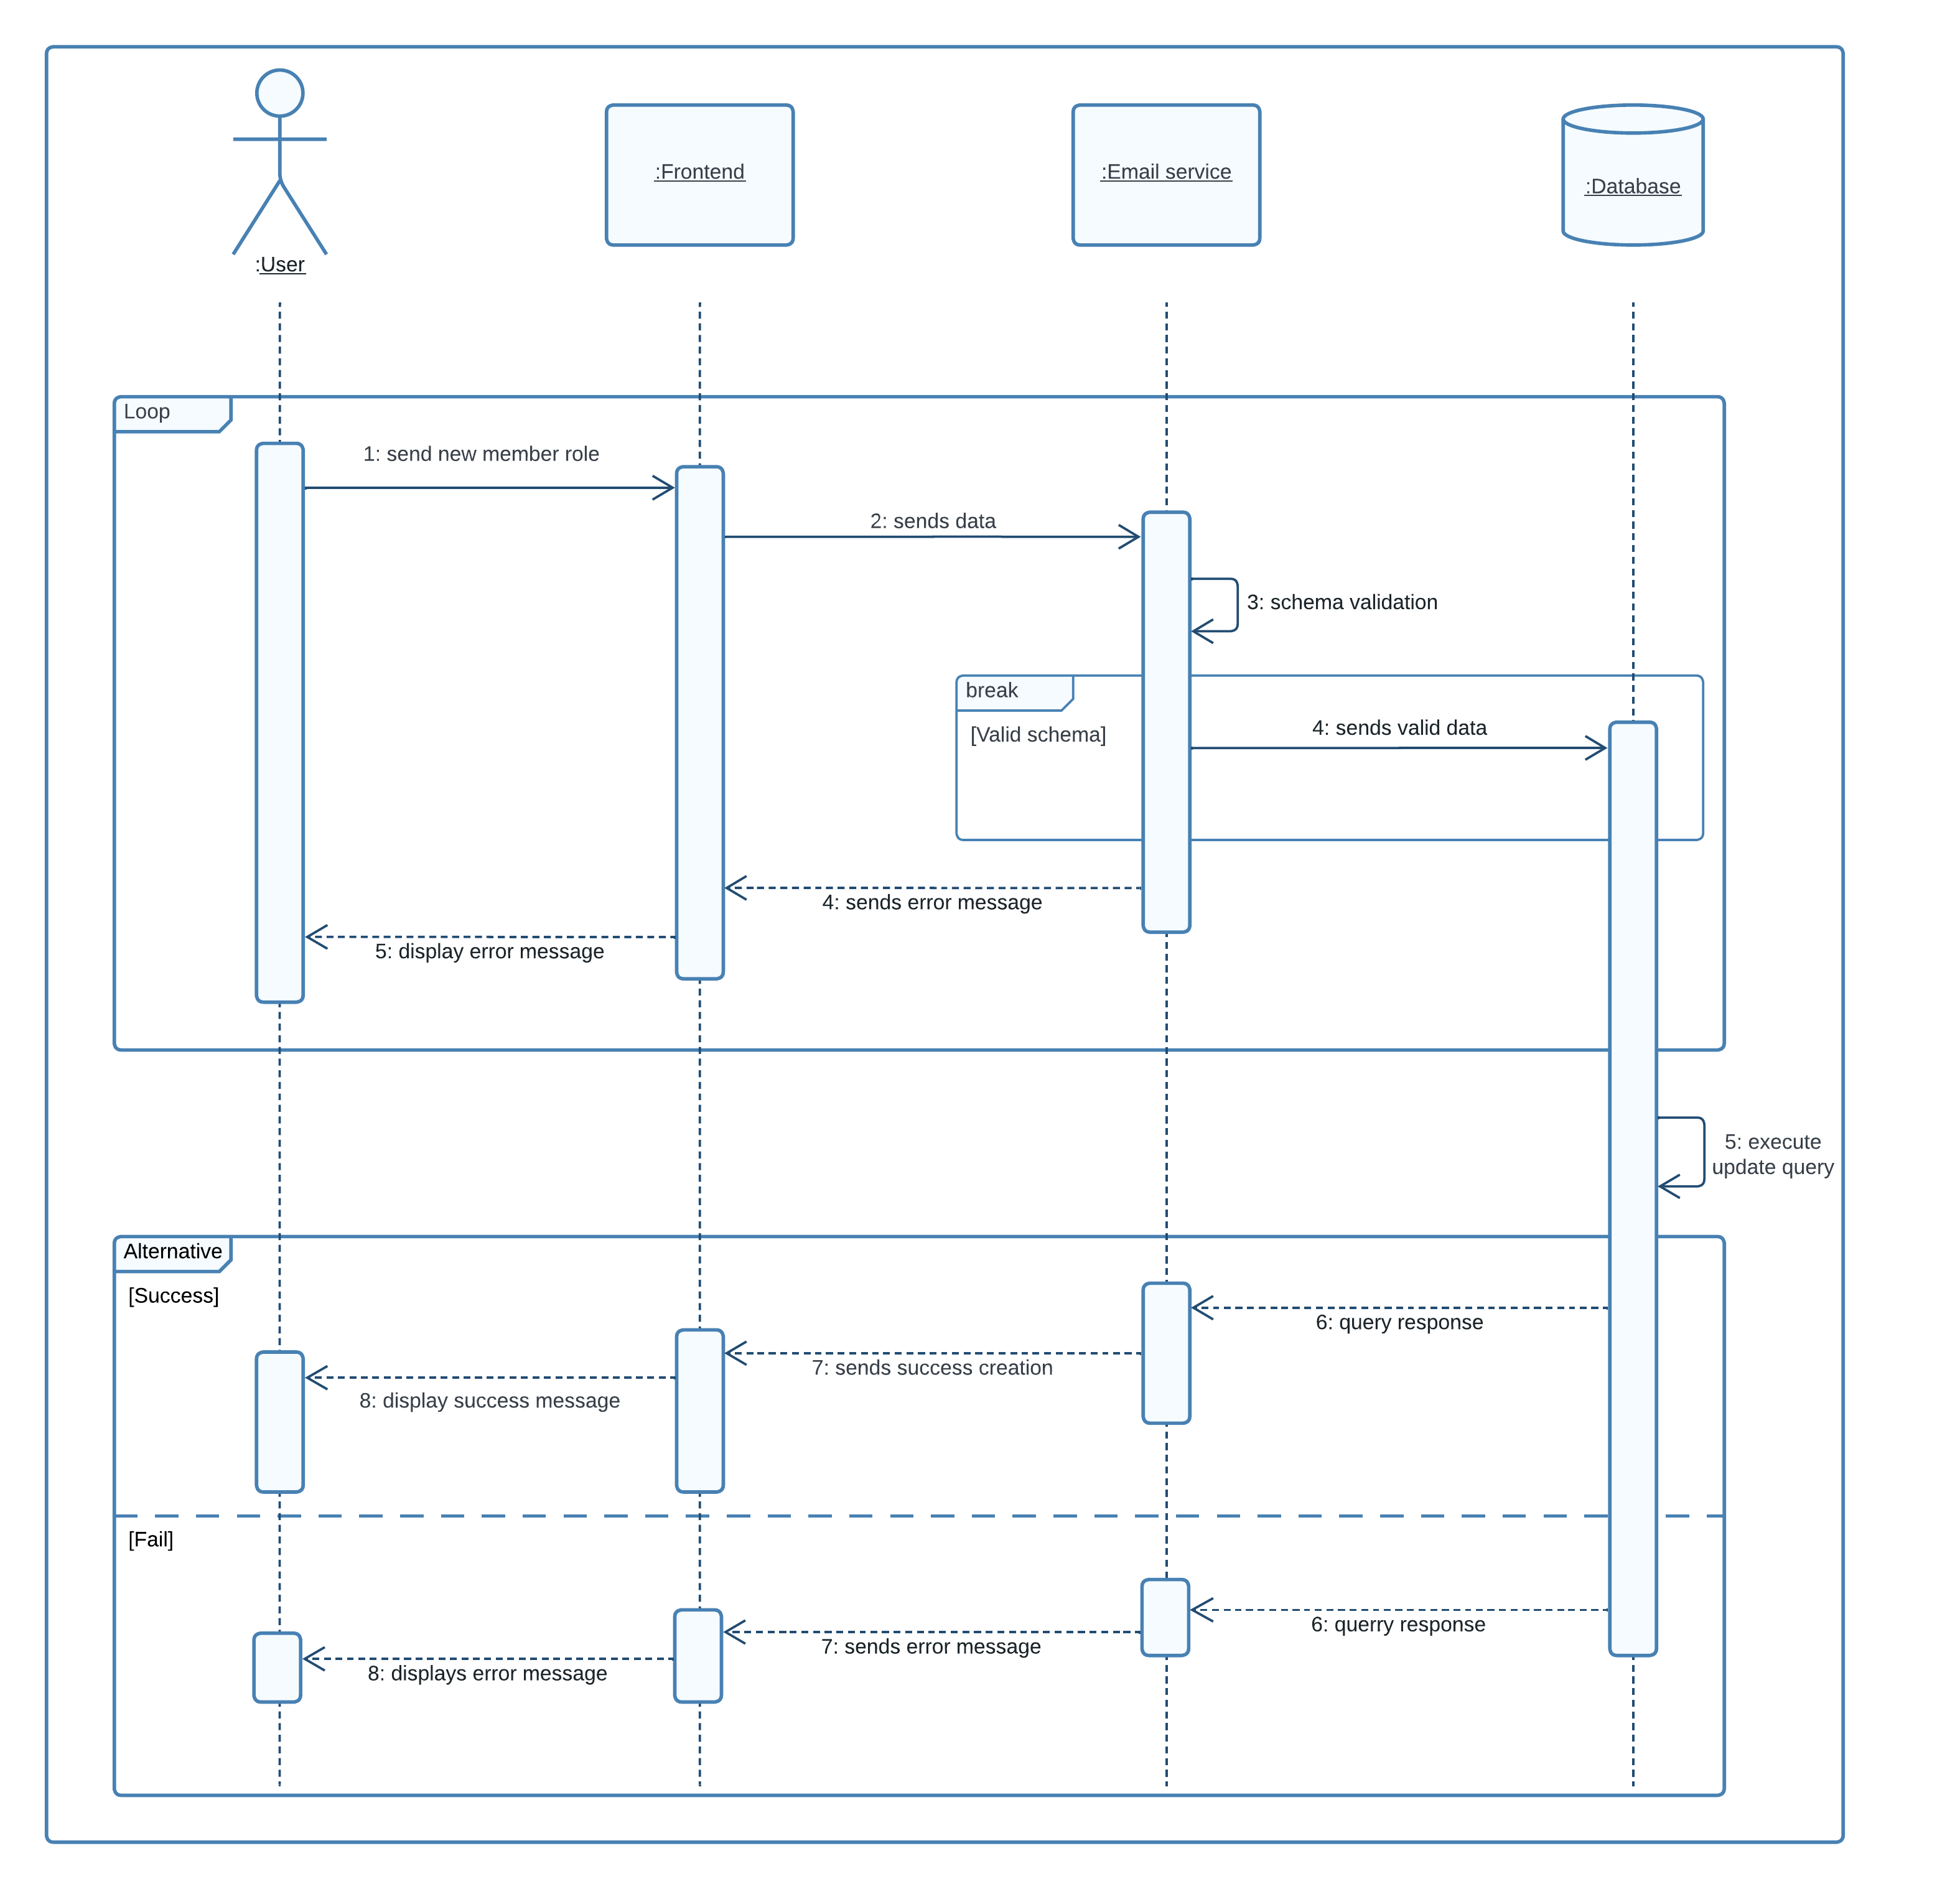
\includegraphics[width=\linewidth]{Images/sprint2/assign roles seq diag.png}
	\caption{ Assign Roles Sequence Diagram}
	\label{fig:Sprint 2 Assign Roles Sequence Diagram}
\end{figure}

\clearpage

\subsubsection{Remove Members Sequence Diagram}

Figure \ref{fig:Sprint 2 Remove Members Sequence Diagram} describes the scenario of the "Remove Members" use case.

\begin{figure}[ht]
	\centering
	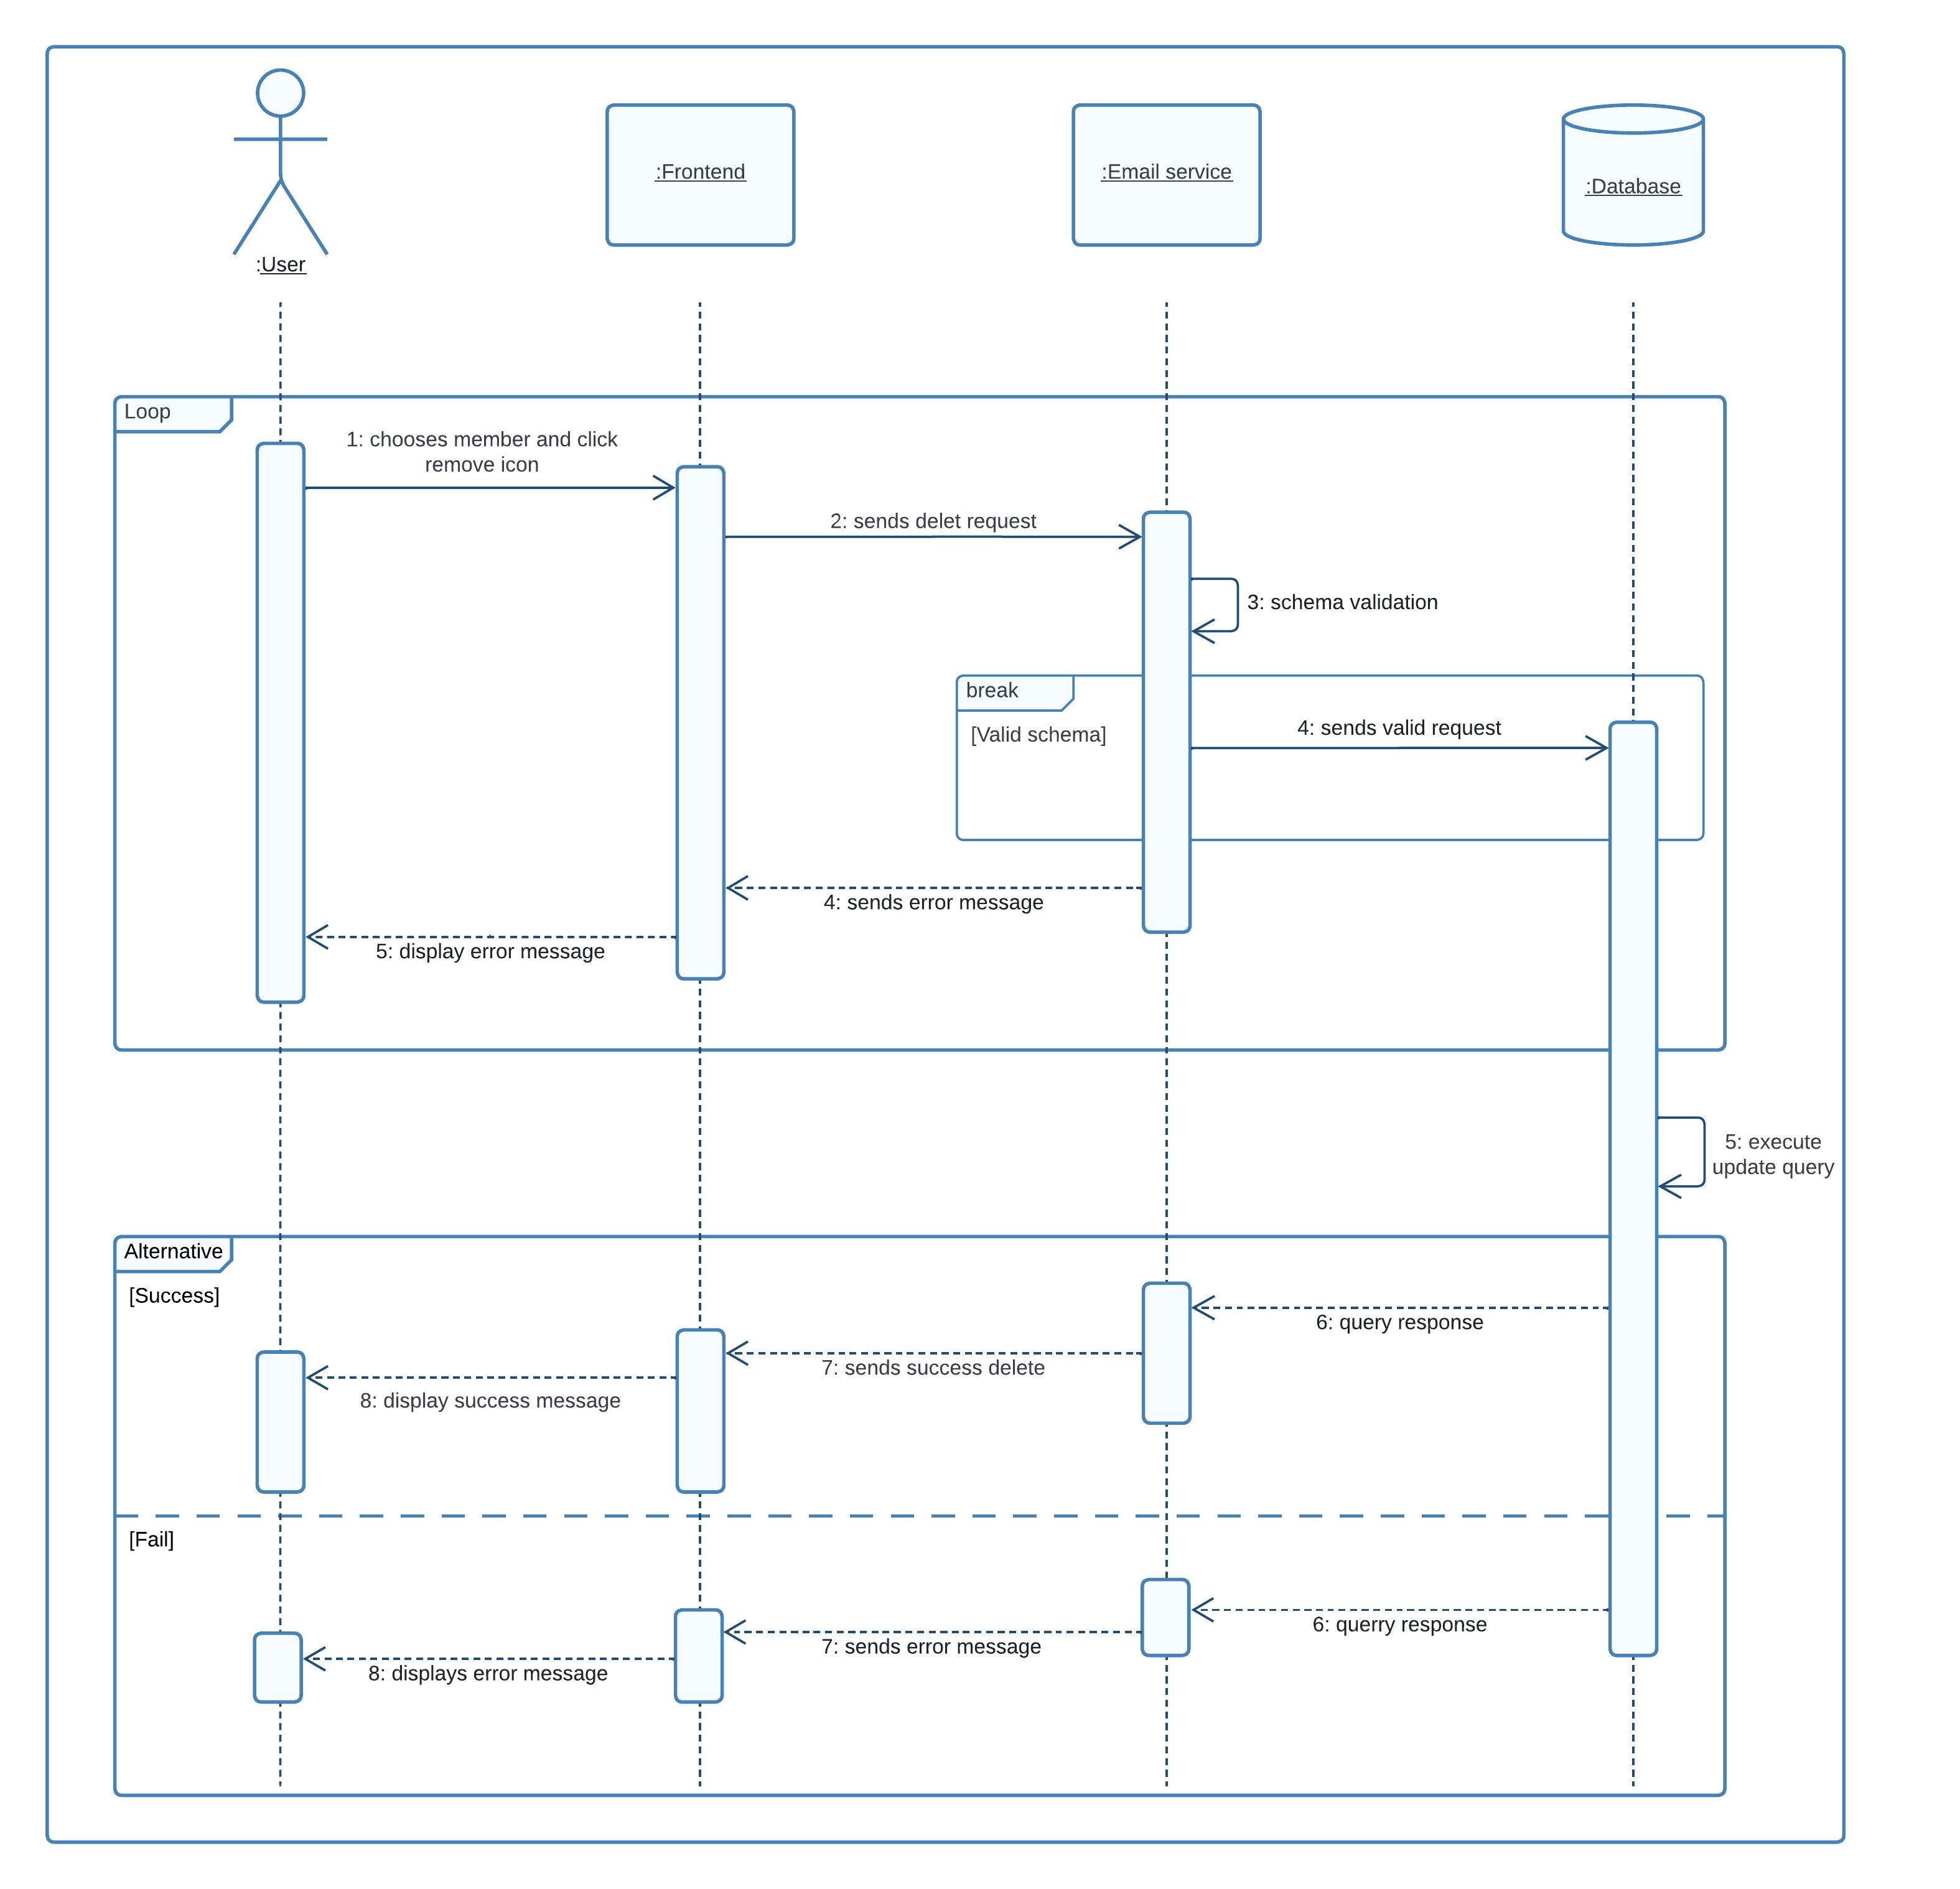
\includegraphics[width=\linewidth]{Images/sprint2/remove member seq diag.png}
	\caption{ Remove Members Sequence Diagram}
	\label{fig:Sprint 2 Remove Members Sequence Diagram}
\end{figure}
